\section{Arbeitsgrundlagen}


\subsection{Messung der Lichtgeschwindigkeit nach Michelson}

In diesem Versuch wird die Lichtgeschwindigkeit nach der Methode von Michelson
(Abbildung  \ref{fig:michelson}) gemessen. Dabei  wird  ein Laserstrahl  durch
verschiedene  Linsen, Spiegeln  und  Blenden  hin- und  zur\"uckgeschickt. Ein
Spiegel, $DS$,  wird mit einem  Motor bei verschiedenen,  bekannten Drehzahlen
rotiert.  Da das Licht endlich schnell ist, wird der Drehspiegel einen anderen
Winkel haben  nach Zur\"uckreflektieren  des Lichtstrahls vom  Endspiegel $ES$
und verursacht somit eine Verschiebung des Zur\"uckkommenden Laserstrahls. Ist
die  Distanz  zwischen  Endspiegel  und  Drehspiegel $f_2  +  S_2$  sowie  die
Drehzahl  $\omega$  bekannt,  so  kann  durch  Messung  der  Verschiebung  die
Lichtgeschwindigkeit berechnet werden.

\begin{figure}[H]
    \center
    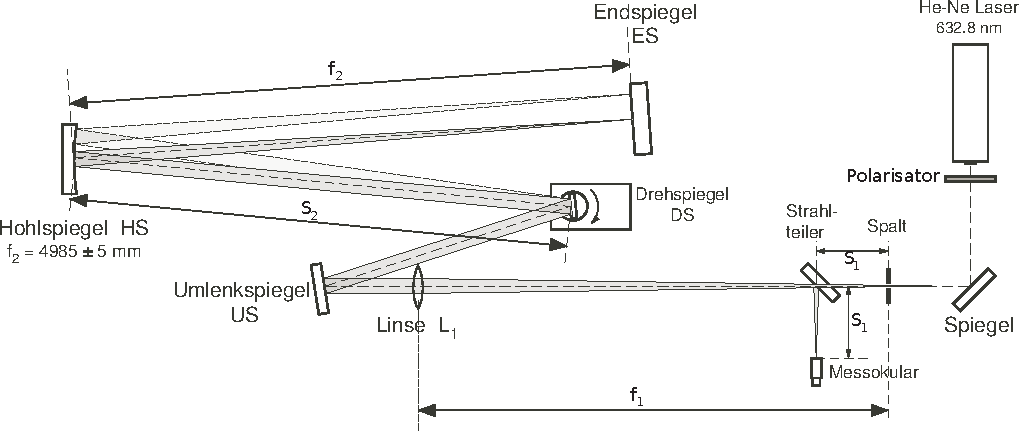
\includegraphics[width=\textwidth]{images/michelson.pdf}
    \caption{Versuchsaufbau nach Michelson. Auszug aus der Aufgabenstellung.}
    \label{fig:michelson}
\end{figure}

Der Versuch  nach Michelson kann mit  einer \"Aquivalenten Linsenkonfiguration
dargestellt werden,  wie in  der Abbildung  \ref{fig:linsenkonfig} ersichtlich
ist.

\begin{figure}[H]
    \center
    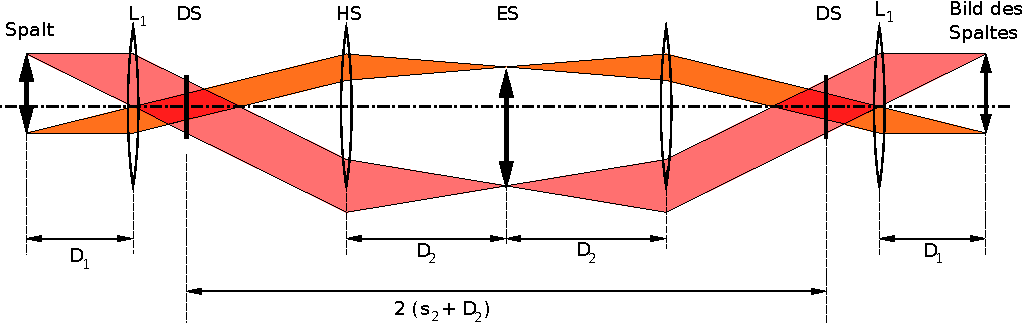
\includegraphics[width=\textwidth]{images/linsenkonfig.pdf}
    \caption{\"Aquivalente Linsenkonfiguration des Versuchs. Auszug aus der Aufgabenstelung}
    \label{fig:linsenkonfig}
\end{figure}

Bei rotierendem Spiegel  findet das vom Endspiegel  zur\"uckkehrende Licht den
Drehspiegel  wegen der  endlichen Laufzeit  um einen  kleinen Winkel  $\delta$
gedreht

\begin{equation}
    \delta = \omega \cdot \Delta t = \omega \cdot \frac{2(S_2 + f_2)}{c}
    \label{eq:delta}
\end{equation}

wobei $\omega$ die Kreisfrequenz des  Drehspiegels und $\Delta t$ die Laufzeit
des Lichtes  vom Drehspiegel  zum Endspiegel  und zur\"uck  bezeichnen.  Diese
Drehung  des  Spiegels  hat  eine  Richtungs\"anderung  der  B\"undelachse  um
den Winkel $2\delta$  (Reflexionsgesetz, Abbildung \ref{fig:reflexionsgesetz},
$\alpha=\alpha' \to  2\delta$) und damit  eine seitliche Verschiebung  $x$ des
Bildes des Spaltes zur Folge.

\begin{figure}[H]
    \center
    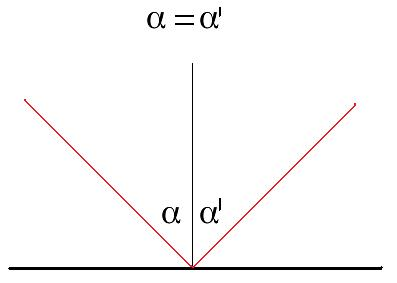
\includegraphics[width=.4\textwidth]{images/reflexionsgesetz.jpg}
    \caption{Reflexionsgesetz}
    \label{fig:reflexionsgesetz}
\end{figure}

F\"ur   das    Verst\"andnis   des   Strahlenganges   ben\"otigen    wir   die
Abbildungsgleichung und den Abbildungsmassstab $\beta$ f\"ur d\"unne Linsen.

\begin{equation}
    \frac{1}{f} = \frac{1}{g} + \frac{1}{b}
    \hspace{15mm}\textrm{und}\hspace{15mm}
    \beta = \frac{B}{G} = \frac{b}{g}
    \label{eq:optik}
\end{equation}

Wobei  $f$  die   Brennweite,  $g$  die  Gegenstandsweite   (Abstand  Linse  -
Gegenstand),   $b$  die   Bildweite,  $B$   die  Bildgr\"osse   und  $G$   die
Gegenstandsgr\"osse bezeichnen.

Da die Kleinwinkeln\"aherung $\sin\theta \approx \tan\theta \approx \theta$ in
unserem Falle sicher zul\"assig ist, gilt
\begin{equation}
    2\delta = \frac{x}{f_1}
\end{equation}
und damit
\begin{equation}
    c = 4\omega \cdot \frac{(S_2 + f_2)f_1}{x}
\end{equation}

Eine   sch\"one  Visualisierung   der  Verschiebung   in  Abh\"angigkeit   des
einstrahlwinkels  kann  in  der Abbildung  \ref{fig:lense-simulation}  gesehen
werden\footcite{ref:linsen-simulation}. Die   weissen   Linien  strahlen   mit
einem  anderen Winkel  als  die  gelbe Linien  in  die  Linse und  verursachen
dementsprechend eine vertikale Verschiebung des Bildes.

\begin{figure}[H]
    \center
    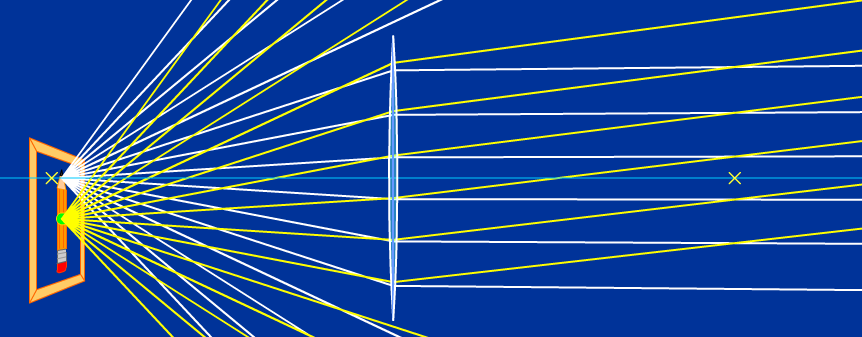
\includegraphics[width=.8\textwidth]{images/lense-simulation.png}
    \caption{Verhalten von Lichtstrahlen bei unterschiedlichen Einstrahlwinkel}
    \label{fig:lense-simulation}
\end{figure}

